\documentclass[a4paper,11pt]{article}

\usepackage[english]{babel}
\usepackage{mathrsfs, amssymb, amsmath, amsthm, enumerate}
\usepackage{verbatim,graphicx,geometry}
%\usetikzlibrary{arrows}
\usepackage[utf8]{inputenc}
\usepackage{authblk}
\usepackage[round]{natbib}
\bibliographystyle{plainnat}

\usepackage{hyperref}

\makeatletter
\def\@biblabel#1{\hspace*{-\labelsep}}
\makeatother
\geometry{left=1in,right=1
in,top=1in,bottom=1in}
\newdimen\dummy
\dummy=\oddsidemargin
\addtolength{\dummy}{72pt}
\marginparwidth=.5\dummy
\marginparsep=.1\dummy


\newcommand{\E}{\mathbb{E}}
\newcommand{\Var}{\mathrm{Var}}
\newcommand{\plim}{\overset{p}{\longrightarrow}}
\newcommand{\dlim}{\overset{d}{\longrightarrow}}

\begin{document}

\section*{Parameter Search}

\begin{table}[h!]
\centering
\begin{tabular}{llll}
\hline \hline
variable & value & objective function & interpretation \\ \hline
$\eta^H$ & 0.15 & 0.026 & New technology benefit \\
$\eta^M$ & 0.03 & 0.026 & New combination benefit \\
$\tau$ & 300 & 0.026 & Shape parameter for idea distribution \\
$\xi$ & 10 & 0.026 & $1/\xi$ is the fraction of viable combinations \\
$\lambda $ & 2.2 & 0.026 & scale parameter of the cost distribution \\
$\kappa $ & 5 & 0.026 & shape parameter of the cost distribution \\
\hline \hline
\end{tabular}
\caption{Current values that minimize the objective function}
\end{table}


\begin{table}[h!]
\centering
\begin{tabular}{llll}
\hline \hline
Column \# & Moment & Model & Data \\ \hline
%1 & Fraction of refinements in 1880 & 28\% & 55\% \\
2 & Fraction of new combinations in 1880 & 45.21\% & 30\% \\
3 & Fraction of new technologies in 1880 & 10.1\% & 10\% \\
%4 & Fraction of refinements in 1930 & 13.38\% & 35\% \\
5 & Fraction of new combinations in 1930 & 64.16\% & 60\% \\
6 & Fraction of new technologies in 1930 & 5.42\% & 3\% \\
7 & Peak of the refinement share & 62.3\% & 60\% \\
8 & Year of the peak in refinement share & 1849 & 1870 \\
\hline \hline
\end{tabular}
\caption{Moments (the missing column numbers are the moments I dropped relative to the old specification). Obs.: column 8 is not included as an argument in the objective function $\Rightarrow$ still under-identified.}
\end{table}


\begin{figure}[h!]
\begin{center}
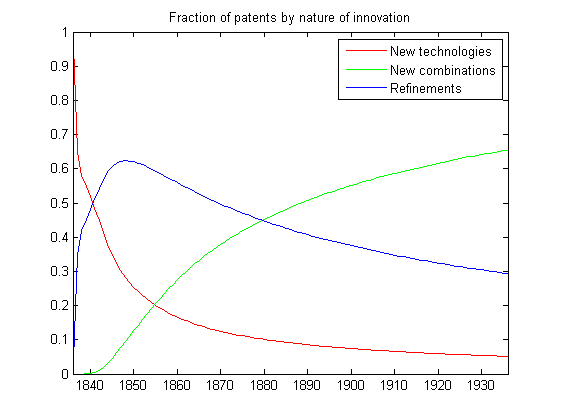
\includegraphics[scale=.8]{fractions_new.png}
\caption{Fraction of patents by type}
\end{center}
\end{figure}

\clearpage

\section*{Sensitivity analysis}

\begin{table}[h!]
\hspace*{-1cm}\begin{tabular}{lllllll}
\hline \hline
\textbf{Parameter changed}&\textbf{NC 1880}&\textbf{NT 1880}&\textbf{NC 1930}&\textbf{NT 1930}&\textbf{Peak of reuse} & \textbf{Year of peak}\\\hline
\textbf{$\eta^H$}&0.25314&0.077351&0.45259&0.040606&0.79891&1851\\\hline
\textbf{$\eta^M$}&0.44517&0.1036&0.63846&0.055556&0.62018&1850\\\hline
\textbf{$\tau$}&0.41794&0.093815&0.61242&0.05038&0.66305&1850\\\hline
\textbf{$\lambda$}&0.56153&0.11383&0.73459&0.061152&0.51344&1848\\\hline
\textbf{$\kappa$}&0.47448&0.10177&0.66667&0.054808&0.6135&1849\\\hline
\textbf{$\xi$}&0.48193&0.10102&0.66175&0.05405&0.59305&1849\\\hline
\textbf{Baseline}&0.4521&0.101&0.6416&0.0542&0.623&1849\\\hline
\textbf{data}&0.3&0.1&0.6&0.03&0.6&1870\\
\hline \hline
\end{tabular}
\caption{Variation in moments given 20\% decrease in parameter values.}
\end{table}

From table 3, $\eta^H$ and $\lambda$ are driving most of the change. $\tau$, $\kappa$ and $\xi$ also seem to have a considerable effect on the fraction of new combinations. $\eta^M$ has the weakest effect in all moments.

\section*{Rate of Growth}

\begin{figure}[h!]
\begin{center}
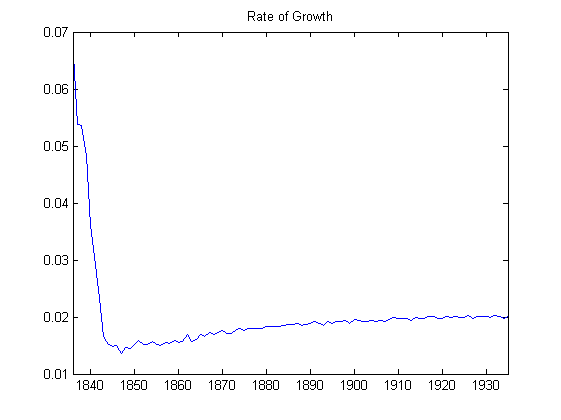
\includegraphics[scale=.8]{growth.png}
\caption{Growth rate of economy}
\end{center}
\end{figure}

Figure 2 has the rate of growth of the economy. It was computed by taking the average patent quality among firms. I chose the number of firms to yield an average growth rate of 2\%, which gave 683 firms. 

Until around 1845, the rate of growth seems to be affected the most by the movement of the fraction of new technologies. This feature can be somewhat ``artificial", happening mainly because we define the fraction of new technologies in 1836 to be equal to 1. Soon after that, this effect fades out and the rate of growth seems to stabilize around 2\%, the historical mean. Note that there is a slight increase in the rate of growth, as the fraction of new combinations increases as well. 

If we zoom in on the rate of growth starting at 1846 instead, we get figure 3:

\begin{figure}[h!]
\begin{center}
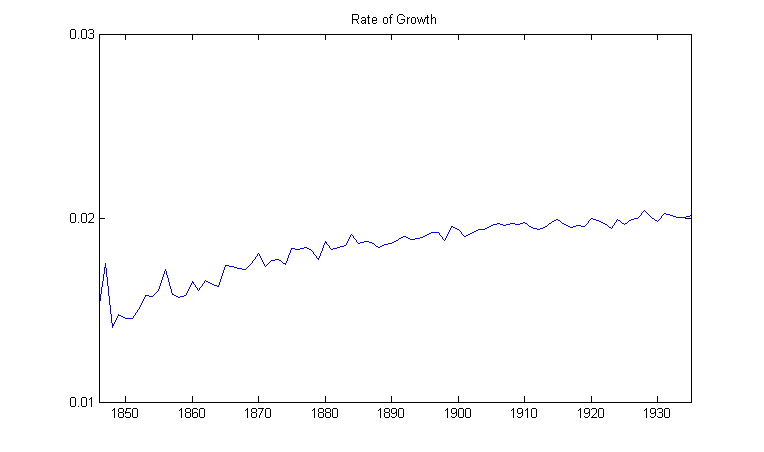
\includegraphics[scale=.8]{growth_zoom.png}
\caption{Growth rate of economy after 1846.}
\end{center}
\end{figure}



\end{document}